% Options for packages loaded elsewhere
\PassOptionsToPackage{unicode}{hyperref}
\PassOptionsToPackage{hyphens}{url}
\PassOptionsToPackage{dvipsnames,svgnames,x11names}{xcolor}
\documentclass[
  11pt,
]{article}
\pdftrailerid{}
\usepackage{xcolor}
\usepackage{amsmath,amssymb}
\setcounter{secnumdepth}{-\maxdimen} % remove section numbering
\usepackage{iftex}
\ifPDFTeX
  \usepackage[T1]{fontenc}
  \usepackage[utf8]{inputenc}
  \usepackage{textcomp} % provide euro and other symbols
\else % if luatex or xetex
  \usepackage{unicode-math} % this also loads fontspec
  \defaultfontfeatures{Scale=MatchLowercase}
  \defaultfontfeatures[\rmfamily]{Ligatures=TeX,Scale=1}
\fi
\usepackage{lmodern}
\ifPDFTeX\else
  % xetex/luatex font selection
\fi
% Use upquote if available, for straight quotes in verbatim environments
\IfFileExists{upquote.sty}{\usepackage{upquote}}{}
\IfFileExists{microtype.sty}{% use microtype if available
  \usepackage[]{microtype}
  \UseMicrotypeSet[protrusion]{basicmath} % disable protrusion for tt fonts
}{}
\makeatletter
\@ifundefined{KOMAClassName}{% if non-KOMA class
  \IfFileExists{parskip.sty}{%
    \usepackage{parskip}
  }{% else
    \setlength{\parindent}{0pt}
    \setlength{\parskip}{6pt plus 2pt minus 1pt}}
}{% if KOMA class
  \KOMAoptions{parskip=half}}
\makeatother
\usepackage{graphicx}
\makeatletter
\newsavebox\pandoc@box
\newcommand*\pandocbounded[1]{% scales image to fit in text height/width
  \sbox\pandoc@box{#1}%
  \Gscale@div\@tempa{\textheight}{\dimexpr\ht\pandoc@box+\dp\pandoc@box\relax}%
  \Gscale@div\@tempb{\linewidth}{\wd\pandoc@box}%
  \ifdim\@tempb\p@<\@tempa\p@\let\@tempa\@tempb\fi% select the smaller of both
  \ifdim\@tempa\p@<\p@\scalebox{\@tempa}{\usebox\pandoc@box}%
  \else\usebox{\pandoc@box}%
  \fi%
}
% Set default figure placement to htbp
\def\fps@figure{htbp}
\makeatother
\setlength{\emergencystretch}{3em} % prevent overfull lines
\providecommand{\tightlist}{%
  \setlength{\itemsep}{0pt}\setlength{\parskip}{0pt}}
% obstruction_preamble.tex — shared house style for ALL papers.
% Engine: pdfLaTeX (portable, no font cache). Injected by pandoc (see makefile).
% pandoc loads fontenc(T1)+inputenc(utf8) before this; hyperref after (so we set
% link colors via pandoc -V flags, not here).

% ---- Fonts & math ----
\IfFileExists{lmodern.sty}{\usepackage{lmodern}}{}   % Latin Modern if present
\usepackage{amsmath,amssymb,amsthm}                  % \mathbb \mathfrak \square ...
\usepackage{microtype}

% ---- Over-wide \boxed kernel statements shrink to fit the text width ----
% A long \boxed{\text{...}} line can exceed \linewidth because \text does not
% line-break in math mode. "max width=\linewidth" scales down ONLY boxes that
% are wider than the text block; short math boxes are left at natural size.
% One place, all papers.
\usepackage{adjustbox}
\let\oboldboxed\boxed
\renewcommand{\boxed}[1]{\adjustbox{max width=\linewidth}{\oboldboxed{#1}}}
\setlength{\emergencystretch}{3em}

% ---- Line breaking for verbatim and code blocks ----
\usepackage{fancyvrb}

% ---- Safe line breaking for typewriter font & long URLs/DOIs ----
\usepackage[htt]{hyphenat}
\usepackage{xurl}
\usepackage[hyphens]{url}


% ---- Flawless fix: literal Unicode (ℓ¹ Φ₁ κ¹ ⊗ →) in TEXT mode ----
% In $...$ these already work; this maps stray text-mode glyphs to math so
% nothing renders blank and you never rewrite source. If a build ever says
% "Unicode character X not set up", add one line here for that glyph.
\usepackage{newunicodechar}
\newcommand{\um}[1]{\ensuremath{#1}}
\newunicodechar{ℓ}{\um{\ell}}
\newunicodechar{Φ}{\um{\Phi}}\newunicodechar{φ}{\um{\varphi}}
\newunicodechar{Ψ}{\um{\Psi}}\newunicodechar{ψ}{\um{\psi}}
\newunicodechar{⇔}{\um{\Leftrightarrow}}
\newunicodechar{Γ}{\um{\Gamma}}\newunicodechar{γ}{\um{\gamma}}
\newunicodechar{Ω}{\um{\Omega}}\newunicodechar{ω}{\um{\omega}}
\newunicodechar{κ}{\um{\kappa}}\newunicodechar{χ}{\um{\chi}}
\newunicodechar{Λ}{\um{\Lambda}}\newunicodechar{λ}{\um{\lambda}}
\newunicodechar{Θ}{\um{\Theta}}\newunicodechar{θ}{\um{\theta}}
\newunicodechar{Δ}{\um{\Delta}}\newunicodechar{δ}{\um{\delta}}
\newunicodechar{Σ}{\um{\Sigma}}\newunicodechar{σ}{\um{\sigma}}
\newunicodechar{Π}{\um{\Pi}}\newunicodechar{π}{\um{\pi}}
\newunicodechar{α}{\um{\alpha}}\newunicodechar{β}{\um{\beta}}
\newunicodechar{ε}{\um{\varepsilon}}\newunicodechar{μ}{\um{\mu}}
\newunicodechar{ρ}{\um{\rho}}\newunicodechar{τ}{\um{\tau}}
\newunicodechar{ν}{\um{\nu}}\newunicodechar{ξ}{\um{\xi}}
\newunicodechar{ζ}{\um{\zeta}}\newunicodechar{η}{\um{\eta}}
\newunicodechar{ℝ}{\um{\mathbb{R}}}\newunicodechar{ℚ}{\um{\mathbb{Q}}}
\newunicodechar{ℤ}{\um{\mathbb{Z}}}\newunicodechar{ℕ}{\um{\mathbb{N}}}
\newunicodechar{ℂ}{\um{\mathbb{C}}}
\newunicodechar{𝒟}{\um{\mathcal{D}}}
\newunicodechar{→}{\um{\to}}\newunicodechar{↦}{\um{\mapsto}}
\newunicodechar{≤}{\um{\leq}}\newunicodechar{≥}{\um{\geq}}
\newunicodechar{≠}{\um{\neq}}\newunicodechar{≈}{\um{\approx}}
\newunicodechar{≅}{\um{\cong}}\newunicodechar{≡}{\um{\equiv}}
\newunicodechar{⊗}{\um{\otimes}}\newunicodechar{⊕}{\um{\oplus}}
\newunicodechar{∘}{\um{\circ}}\newunicodechar{∂}{\um{\partial}}
\newunicodechar{∇}{\um{\nabla}}\newunicodechar{∑}{\um{\sum}}
\newunicodechar{∏}{\um{\prod}}\newunicodechar{∞}{\um{\infty}}
\newunicodechar{⊆}{\um{\subseteq}}\newunicodechar{⊂}{\um{\subset}}
\newunicodechar{⊇}{\um{\supseteq}}\newunicodechar{∈}{\um{\in}}
\newunicodechar{∉}{\um{\notin}}\newunicodechar{∩}{\um{\cap}}
\newunicodechar{∪}{\um{\cup}}\newunicodechar{∖}{\um{\setminus}}
\newunicodechar{∅}{\um{\varnothing}}\newunicodechar{⊥}{\um{\perp}}
\newunicodechar{∀}{\um{\forall}}\newunicodechar{∃}{\um{\exists}}
\newunicodechar{±}{\um{\pm}}\newunicodechar{×}{\um{\times}}\newunicodechar{−}{\um{-}}
\newunicodechar{·}{\um{\cdot}}\newunicodechar{√}{\um{\surd}}
\newunicodechar{⟨}{\um{\langle}}\newunicodechar{⟩}{\um{\rangle}}
\newunicodechar{≪}{\um{\ll}}\newunicodechar{≫}{\um{\gg}}
\newunicodechar{∝}{\um{\propto}}\newunicodechar{≜}{\um{\triangleq}}
\newunicodechar{⇒}{\um{\Rightarrow}}\newunicodechar{⇐}{\um{\Leftarrow}}
\newunicodechar{∧}{\um{\wedge}}\newunicodechar{∨}{\um{\vee}}
\newunicodechar{⟺}{\um{\iff}}\newunicodechar{□}{\um{\square}}
\newunicodechar{⊔}{\um{\sqcup}}\newunicodechar{…}{\dots}\newunicodechar{‖}{\um{\Vert}}
\newunicodechar{▼}{\um{\blacktriangledown}}\newunicodechar{«}{\guillemotleft}\newunicodechar{»}{\guillemotright}
\newunicodechar{─}{--}\newunicodechar{│}{|}\newunicodechar{┌}{+}\newunicodechar{┐}{+}\newunicodechar{┼}{+}
\newunicodechar{═}{=}\newunicodechar{║}{\um{\parallel}}\newunicodechar{̄}{\={}}
\newunicodechar{⟹}{\um{\implies}}\newunicodechar{⟸}{\um{\impliedby}}
\newunicodechar{⁰}{\textsuperscript{0}}\newunicodechar{¹}{\textsuperscript{1}}
\newunicodechar{²}{\textsuperscript{2}}\newunicodechar{³}{\textsuperscript{3}}
\newunicodechar{⁴}{\textsuperscript{4}}\newunicodechar{⁵}{\textsuperscript{5}}
\newunicodechar{⁶}{\textsuperscript{6}}\newunicodechar{⁷}{\textsuperscript{7}}
\newunicodechar{⁸}{\textsuperscript{8}}\newunicodechar{⁹}{\textsuperscript{9}}
\newunicodechar{⁻}{\textsuperscript{-}}\newunicodechar{⁺}{\textsuperscript{+}}
\newunicodechar{ⁿ}{\textsuperscript{n}}
\newunicodechar{₀}{\textsubscript{0}}\newunicodechar{₁}{\textsubscript{1}}\newunicodechar{ᵀ}{\textsuperscript{T}}
\newunicodechar{₂}{\textsubscript{2}}\newunicodechar{₃}{\textsubscript{3}}
\newunicodechar{ₜ}{\textsubscript{t}}\newunicodechar{ₑ}{\textsubscript{e}}\newunicodechar{ₙ}{\textsubscript{n}}

% ---- Geometry & spacing ----
\usepackage{geometry}\geometry{letterpaper,margin=1in}
\setlength{\parindent}{0pt}\setlength{\parskip}{0.55\baselineskip}\linespread{1.04}

% ---- Palette ----
\usepackage{xcolor}
\definecolor{oblink}{HTML}{1A4D8F}\definecolor{obrule}{HTML}{C2CCD6}
\definecolor{obboxbg}{HTML}{F6F8FA}
\definecolor{obproven}{HTML}{1B7F4B}   % PROVEN / DERIVED / STANDARD
\definecolor{obconj}{HTML}{B45309}     % CONJECTURE / OPEN / FALSE
\definecolor{obdef}{HTML}{6B21A8}      % DEFINITION / INTERPRETIVE
\definecolor{obneutral}{HTML}{475569}

% ---- Headings ----
\usepackage{titlesec}
\titleformat{\section}{\Large\bfseries}{\thesection}{0.6em}{}
\titleformat{\subsection}{\large\bfseries}{\thesubsection}{0.6em}{}
\titleformat{\subsubsection}{\normalsize\bfseries}{\thesubsubsection}{0.6em}{}
\titlespacing*{\section}{0pt}{1.4em}{0.5em}
\titlespacing*{\subsection}{0pt}{1.1em}{0.4em}

% ---- Theorem environments (for when you adopt semantic theorems) ----
\theoremstyle{plain}
\newtheorem{theorem}{Theorem}[section]
\newtheorem{lemma}[theorem]{Lemma}
\newtheorem{proposition}[theorem]{Proposition}
\newtheorem{corollary}[theorem]{Corollary}
\newtheorem{conjecture}[theorem]{Conjecture}
\theoremstyle{definition}\newtheorem{definition}[theorem]{Definition}
\theoremstyle{remark}\newtheorem*{remark}{Remark}

% ---- Blockquotes -> one uniform left-ruled callout ----
% pandoc wraps every `>` block (your theorems, Status notes, caveats) in `quote`.
\usepackage{mdframed}
\renewenvironment{quote}{%
  \begin{mdframed}[linewidth=0pt,leftline=true,linecolor=obrule,
    rightline=false,topline=false,bottomline=false,
    innerleftmargin=1em,innerrightmargin=0.8em,innertopmargin=0.5em,
    innerbottommargin=0.5em,skipabove=0.6em,skipbelow=0.6em,
    backgroundcolor=obboxbg]\small}{\end{mdframed}}

% ---- Claim-type tag macro ----
\newcommand{\claimtag}[2]{{\small\sffamily\bfseries\color{#1}[#2]}}

% ---- Inline code / file references -> standard breakable typewriter font ----
\DeclareRobustCommand{\texttt}[1]{%
  \ifmmode
    \mathtt{#1}%
  \else
    {\ttfamily\small\renewcommand{\_}{\symbol{95}\allowbreak}#1}%
  \fi}



% ---- "What this does not claim" box ----
\usepackage[most]{tcolorbox}
\newtcolorbox{nonclaim}{colback=obboxbg,colframe=obrule,boxrule=0.6pt,arc=2pt,
  left=1em,right=1em,top=0.5em,bottom=0.5em,
  title={What this does not claim},fonttitle=\bfseries,
  coltitle=black,colbacktitle=obboxbg}

% ---- Tables ----
\usepackage{booktabs}\renewcommand{\arraystretch}{1.15}
\usepackage{etoolbox}
% Compact tables, and let over-long \mathsf{CamelCase} status identifiers wrap
% inside cells. In math, \mathsf{ContinuumShadowBecomesFakeAuthority} is a single
% unbreakable atom and overruns narrow pandoc columns. Scoped to tables only, we
% re-render \mathsf as a sequence of per-word \mathsf atoms split before each
% interior capital and joined by \allowbreak, so the identifier wraps at the math
% top level (an \allowbreak between atoms IS a legal break in inline math; a text
% \mbox/\seqsplit is not). Also shrink the table font and tighten column padding.
% Body math is untouched; table cells carry only plain ASCII identifiers, so the
% splitter is emoji-safe. One place, all papers.
\let\obmathsforig\mathsf
\ExplSyntaxOn
\tl_new:N \l__obt_run_tl
\int_new:N \l__obt_i_int
\cs_new_protected:Npn \__obt_emit:
  {
    \tl_if_empty:NF \l__obt_run_tl
      {
        \int_compare:nNnT { \l__obt_i_int } > { 1 } { \allowbreak }
        \exp_args:NV \obmathsforig \l__obt_run_tl
        \int_incr:N \l__obt_i_int
        \tl_clear:N \l__obt_run_tl
      }
  }
\cs_new_protected:Npn \obtablesf #1
  {
    \tl_clear:N \l__obt_run_tl
    \int_set:Nn \l__obt_i_int { 1 }
    \tl_map_inline:nn {#1}
      {
        \str_if_eq:eeT { \str_uppercase:n {##1} } {##1}
          { \str_if_eq:eeF { \str_lowercase:n {##1} } {##1} { \__obt_emit: } }
        \tl_put_right:Nn \l__obt_run_tl {##1}
      }
    \__obt_emit:
  }
\ExplSyntaxOff
\AtBeginEnvironment{longtable}{\small\setlength{\tabcolsep}{4pt}\let\mathsf\obtablesf}
\AtBeginEnvironment{tabular}{\let\mathsf\obtablesf}

% ---- Title block polish (pandoc \maketitle) ----
% Title and subtitle both centered under each other. Body metadata stays plain
% roman (never a monospaced identity dump). Public monographs must not put
% internal programme IDs (PO-xxx, GS-xxx, …) in the title line.
\usepackage{titling}
\newcommand{\obsubtitle}{}
% Capture pandoc's \subtitle{...} (provide later is a no-op once this is defined).
\newcommand{\subtitle}[1]{\gdef\obsubtitle{#1}}
\pretitle{\begin{center}\LARGE\bfseries}
\posttitle{%
  \par
  \ifx\obsubtitle\empty\else
    \vskip0.4em
    {\large\itshape \obsubtitle\par}%
  \fi
  \end{center}\vskip0.75em}
\preauthor{\begin{center}\large}\postauthor{\par\end{center}}
\predate{\begin{center}\normalsize}\postdate{\par\end{center}\vskip0.5em\hrule\vskip1em}

% ---- Status-box markers (emoji rendered as text glyphs; one place, all papers) ----
\newunicodechar{§}{\S}
\newunicodechar{–}{--}
\newunicodechar{—}{---}
\newunicodechar{‘}{`}
\newunicodechar{’}{'}
\newunicodechar{“}{``}
\newunicodechar{”}{''}
\newunicodechar{✅}{\um{\checkmark}}
\newunicodechar{⚠}{\textbf{!}}
\newunicodechar{☣}{\um{\boxtimes}}
\newunicodechar{⊣}{\um{\dashv}}
\newunicodechar{🔷}{\textcolor{oblink}{\um{\blacklozenge}}}
\newunicodechar{️}{}
\usepackage{bookmark}
\IfFileExists{xurl.sty}{\usepackage{xurl}}{} % add URL line breaks if available
\urlstyle{same}
\hypersetup{
  pdftitle={Local Green, Global Red II: Organizational Evaluator Gluing},
  pdfauthor={Jeremy H. Carroll},
  colorlinks=true,
  linkcolor={oblink},
  filecolor={Maroon},
  citecolor={oblink},
  urlcolor={oblink},
  pdfcreator={LaTeX via pandoc}}

\title{Local Green, Global Red II: Organizational Evaluator Gluing}
\author{Jeremy H. Carroll}
\date{\textbf{Date:} 2026-10-15\\
\textbf{Version:} 1.3.1\\}

\begin{document}
\maketitle
\begin{abstract}
Local checks need not compose into a global check. We study this gap in
a finite Boolean model with local evaluators, a global evaluator, and
their signed disagreement. The negative value is exactly the
local-green/global-red configuration. A weak representation that
recovers the global verdict does not imply evaluator factorization,
while product sufficiency---requiring the recovered global coordinate to
equal the local-pass product---is equivalent to factorization. We
separate this arithmetic from three declared governance prerequisites
and formalize the carrier obstruction: a global evaluator varying inside
a local carrier class cannot factor through the corresponding quotient,
formalizing the standard requirement that functions descending to
equivalence classes respect their identifications. Lean 4 checks the
finite theorems; Python supplies executable audits, falsifiers, figures,
and a tested notebook.
\end{abstract}

\subsection{1. The composition problem}\label{the-composition-problem}

While Part I formalizes evaluated path kernels for composed agent
workflows under proposal-weighted trajectories, Part II studies the
organizational gluing boundary, separating evaluator factorization,
representation sufficiency, and governance prerequisites under
Conway-style organizational interfaces.

Suppose a workflow crosses an interface. Each local unit has a Boolean
evaluator

\[
E_i:X\to\{0,1\},
\]

and the composed outcome has a Boolean evaluator

\[
E_G:X\to\{0,1\}.
\]

For a trace \(x\), write

\[
L(x)=\prod_{i=1}^{n}E_i(x), \qquad
\Delta_E(x)=E_G(x)-L(x).
\]

Because both terms are Boolean,

\[
\Delta_E(x)\in\{-1,0,1\}.
\]

Lean evidence: claim-ledger row \textbf{M1}.

The four Boolean inputs have distinct readings:

\begin{itemize}
\item
  \((E_G,L)=(0,1)\) gives \(\Delta_E=-1\): every local evaluator passes
  and the global evaluator fails.
\item
  \((E_G,L)=(0,0)\) gives \(\Delta_E=0\): agreement at failure.
\item
  \((E_G,L)=(1,1)\) gives \(\Delta_E=0\): agreement at success.
\item
  \((E_G,L)=(1,0)\) gives \(\Delta_E=1\): a global pass despite a local
  failure.
\end{itemize}

Thus zero defect means agreement, not success. This small distinction
prevents the phrase ``global green'' from silently replacing the
equation \(E_G=L\).

\begin{figure}
\centering
\pandocbounded{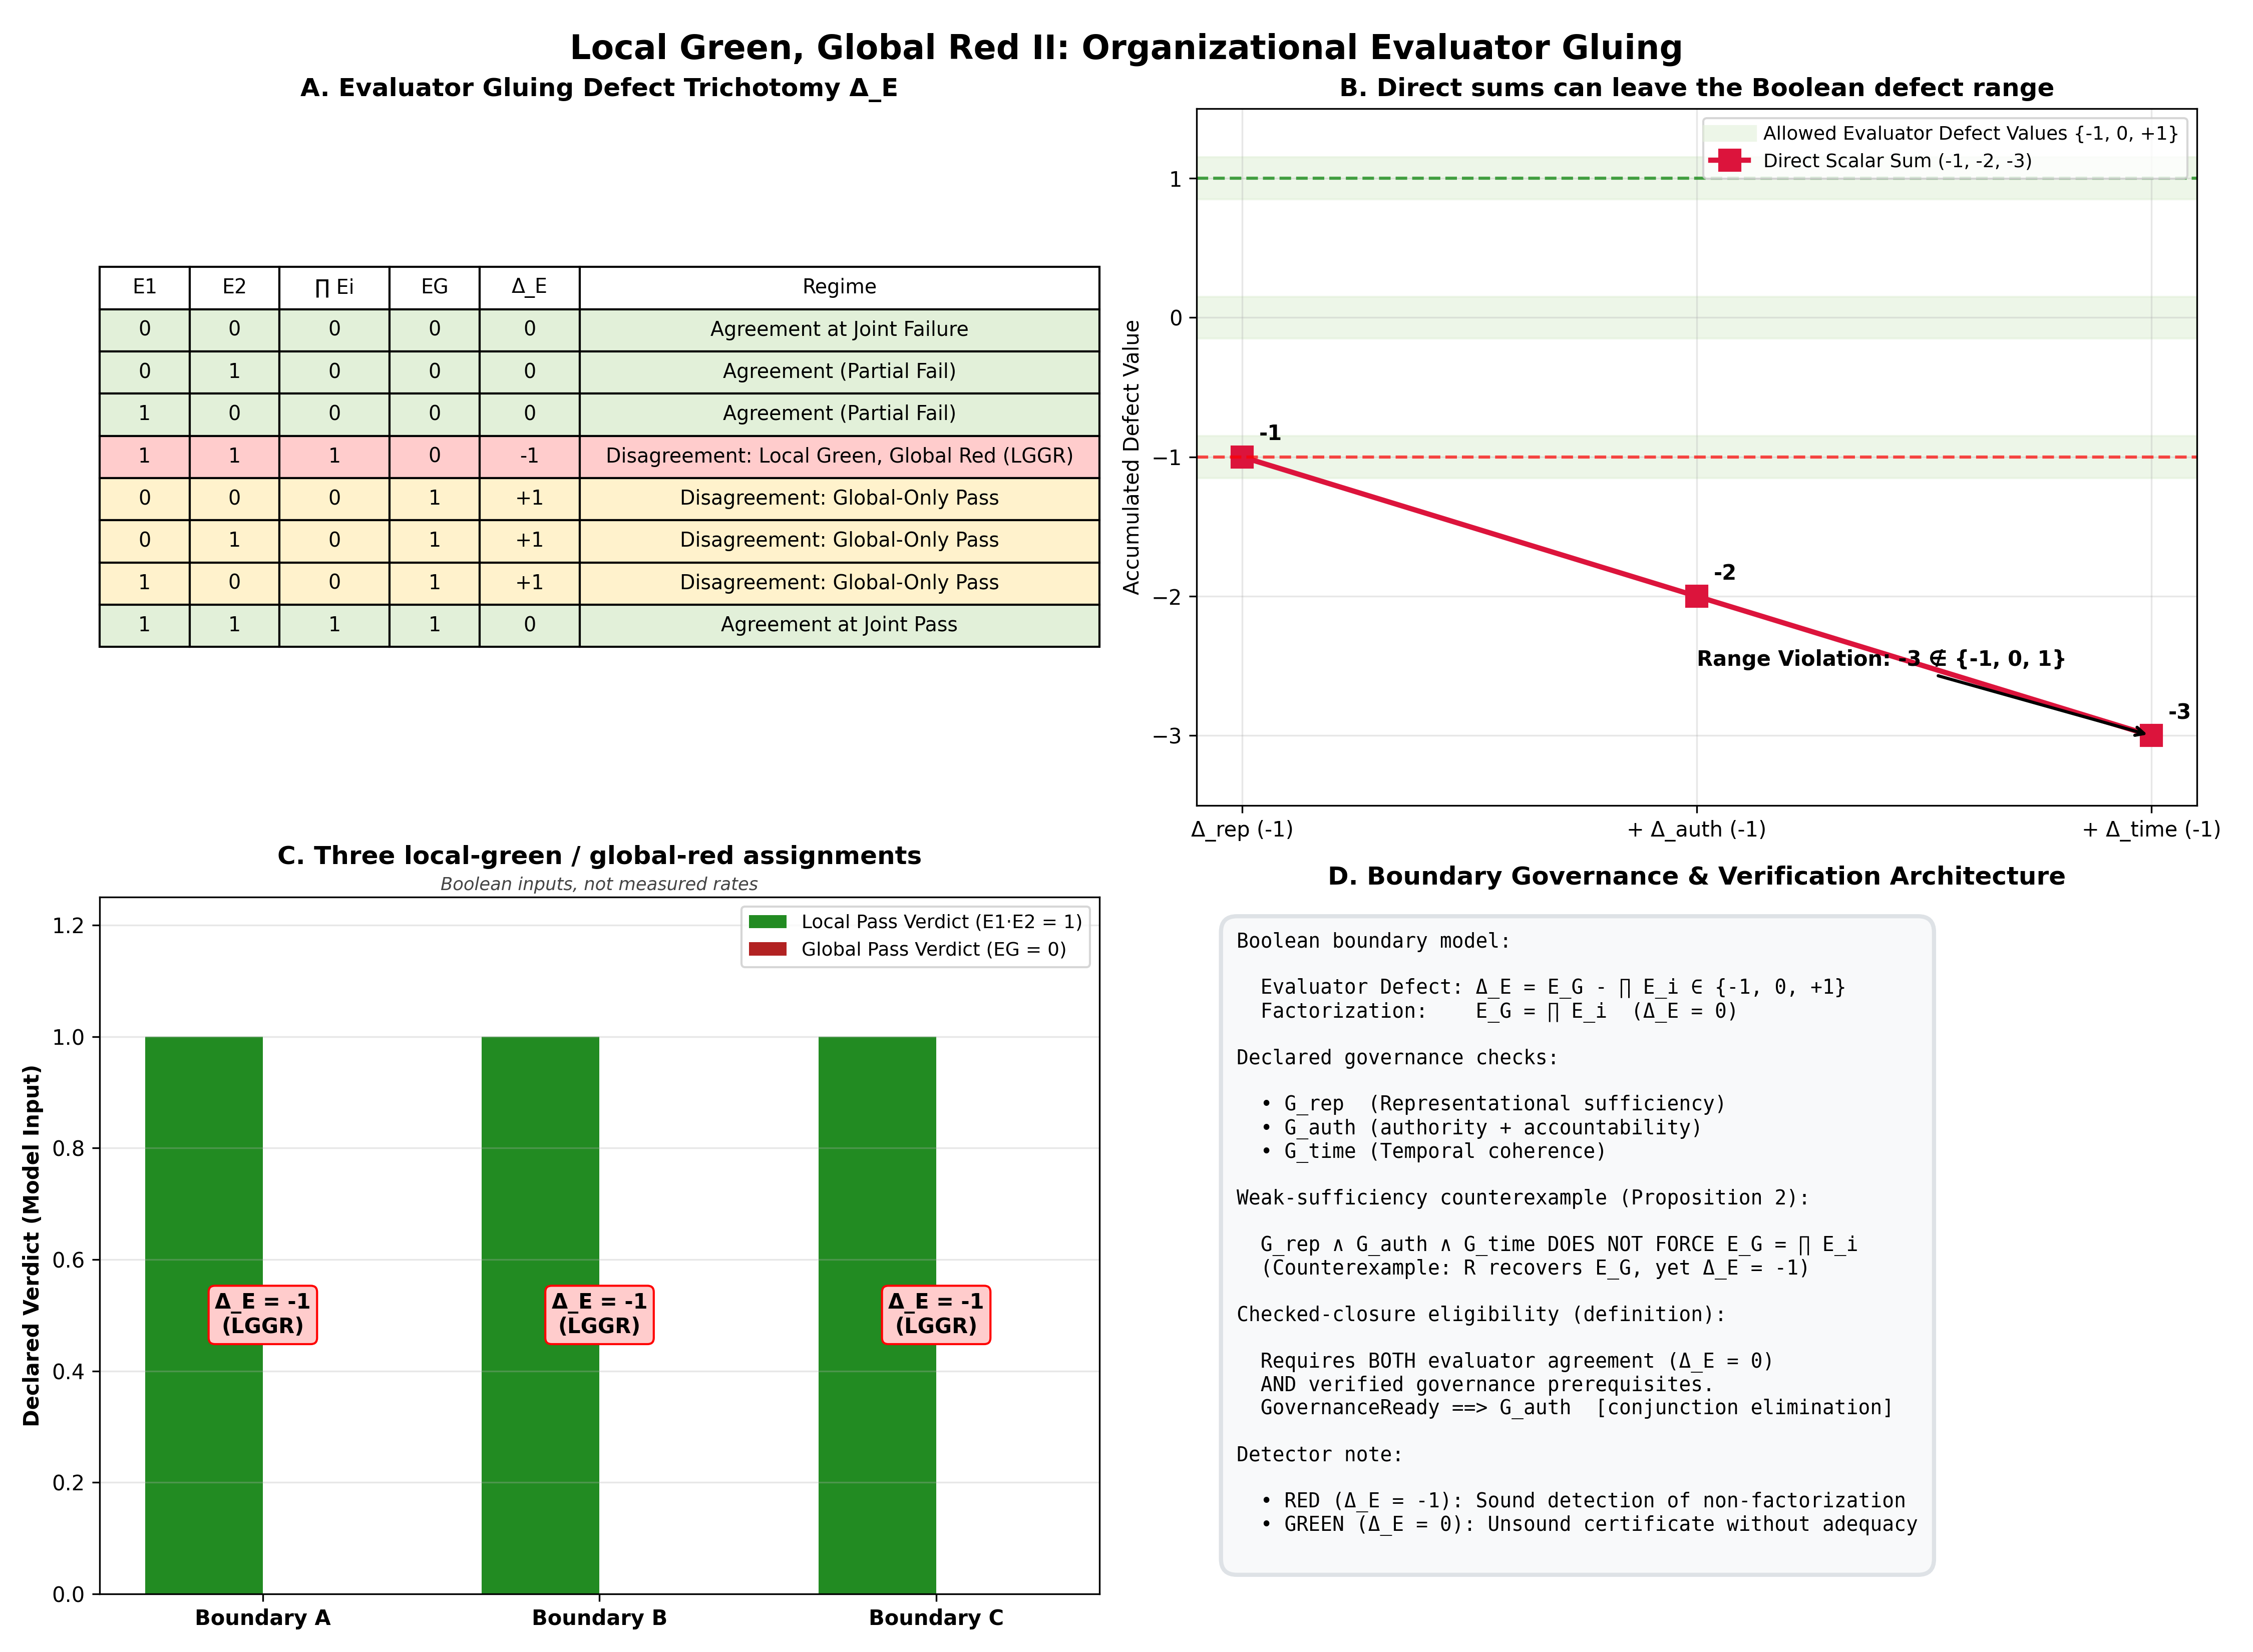
\includegraphics[keepaspectratio,alt={Truth table and boundary model}]{public_export/figure_1_organizational_cut_architecture.png}}
\caption{Truth table and boundary model}
\end{figure}

\subsection{2. Exact finite results}\label{exact-finite-results}

\subsubsection{2.1 Local green and global
red}\label{local-green-and-global-red}

\textbf{Proposition 1.} For Boolean \(E_G\) and \(L\),

\[
\Delta_E=-1 \quad\Longleftrightarrow\quad E_G=0\ \text{and}\ L=1.
\]

\textbf{Proof.} There are four Boolean pairs. Direct evaluation gives
defects \(0,1,-1,0\) for \((E_G,L)=(0,0),(1,0),(0,1),(1,1)\),
respectively. Only \((0,1)\) gives \(-1\), which yields the proposition.

Lean evidence: claim-ledger row \textbf{M2}.

\subsubsection{2.2 Weak representation does not imply
factorization}\label{weak-representation-does-not-imply-factorization}

Let a boundary representation be

\[
R(x)=(E_1(x),E_2(x),E_G(x)).
\]

Call it \emph{weakly sufficient} when its third coordinate recovers
\(E_G\). This condition says nothing about whether \(E_G=E_1E_2\).

\textbf{Proposition 2.} Weak sufficiency, an owner flag, and temporal
coherence do not imply evaluator factorization.

\textbf{Witness.} Take

\[
E_1=1,\quad E_2=1,\quad E_G=0,\quad
R=(1,1,0),\quad G_{\mathrm{auth}}=G_{\mathrm{time}}=1.
\]

The representation recovers \(E_G\), but \(E_G=0\ne1=E_1E_2\). Hence
\(\Delta_E=-1\).

Lean evidence: claim-ledger row \textbf{M3}.

Define \emph{product sufficiency} by requiring the recovered global
coordinate to equal the local product. Under weak sufficiency this is
exactly evaluator factorization:

\[
R_3=E_1E_2 \quad\Longleftrightarrow\quad E_G=E_1E_2.
\]

The Python census evaluates this equivalence on every 8-bit Boolean
boundary. Lean evidence: claim-ledger row \textbf{M4}.

\subsubsection{2.3 Zero defect can be
uninformative}\label{zero-defect-can-be-uninformative}

On a finite sample of traces, call a detector \emph{product-collapsing}
when its complete local product copies the global evaluator:

\[
L(x)=E_G(x)\ \text{for every sampled }x
\quad\Longrightarrow\quad
\Delta_E(x)=0\ \text{on the sample}.
\]

A detector can therefore report agreement by construction. Copying
\(E_G\) into only one local validator is not enough: if another
validator fails on a trace where \(E_G=1\), then the complete product is
zero and the premise above fails. Conversely, a copied validator
together with passing peer validators does make the product equal
\(E_G\). The Lean theorem recorded in row \textbf{M7} checks the product
identity and its all-other-pass specialization. The Python audit checks
the complete product on the supplied nonempty sample, including the
failing-peer counterexample.

Zero defect also occurs when \(E_G=L=0\), so it cannot by itself certify
a passing outcome. Lean checks the counterexample recorded in row
\textbf{M6}.

\subsubsection{2.4 Scalar defects are not additive
channels}\label{scalar-defects-are-not-additive-channels}

Three legal defect values need not have a legal sum:

\[
(-1)+(-1)+(-1)=-3\notin\{-1,0,1\}.
\]

Therefore channel labels such as representation, ownership, and timing
cannot be added as though each were an independent copy of \(\Delta_E\).
Lean evidence is recorded in row \textbf{M5}.

The Python package includes Shapley attribution as an optional
descriptive alternative for a user-supplied coalitional value function.
That computation is an implementation feature, not part of the Lean
result.

\subsection{3. The carrier-class
obstruction}\label{the-carrier-class-obstruction}

The previous propositions use only Boolean arithmetic. A second question
is whether the global evaluator depends solely on the local information
retained at a boundary.

Let a composed trace be \(c=(a,b)\), with local carrier maps
\(\pi_1:A\to P\) and \(\pi_2:B\to Q\). Define

\[
J(c)=(\pi_1(a),\pi_2(b)).
\]

Two traces are locally indistinguishable when their joint carriers
agree. Let \(A\times B/{\sim_J}\) be the quotient by this relation.

\textbf{Theorem 3 (carrier mixing blocks factorization).} If traces
\(c,c'\) satisfy

\[
J(c)=J(c') \qquad\text{and}\qquad E_G(c)\ne E_G(c'),
\]

then there is no function

\[
F:(A\times B/{\sim_J})\to\{0,1\}
\]

such that \(F([x])=E_G(x)\) for every trace \(x\).

\textbf{Proof.} Equality \(J(c)=J(c')\) gives \([c]=[c']\) in the
quotient. Any function on quotient classes must therefore satisfy
\(F([c])=F([c'])\). If it represented \(E_G\), this would give
\(E_G(c)=E_G(c')\), contrary to the hypothesis.

Lean evidence: claim-ledger row \textbf{M8}. Its only nonlogical
dependency in the axiom census is the standard quotient soundness
principle \texttt{Quot.sound}.

For this consequence, assume the local evaluators are carrier-local:
there are functions \(e_1:P\to\{0,1\}\) and \(e_2:Q\to\{0,1\}\) such
that the two local verdicts are \(e_1(\pi_1(a))\) and \(e_2(\pi_2(b))\).
Equality of joint carriers then transports both local verdicts.

If both local evaluators pass on one of these equal carrier classes,
local pass status transports to the other trace. Since the global
Boolean values differ, one of the traces has global value zero and hence
defect \(-1\). Lean checks this consequence in row \textbf{M9}. Finite
traces of this form are evaluated by \texttt{quotient\_factor\_table}
and \texttt{negative\_defect\_witness}.

\newpage

\subsection{4. Organizational
interpretation}\label{organizational-interpretation}

For an organizational boundary, the local evaluators may represent
unit-level acceptance tests and \(E_G\) an end-to-end outcome test. We
record three Boolean prerequisites:

\[
G_{\mathrm{rep}},\qquad G_{\mathrm{auth}},\qquad G_{\mathrm{time}}.
\]

\begin{itemize}
\tightlist
\item
  \(G_{\mathrm{rep}}\): the boundary record retains the information
  required by its declared checks.
\item
  \(G_{\mathrm{auth}}\): an identified owner has both power to change
  the interface and accountability for the global evaluator.
\item
  \(G_{\mathrm{time}}\): local and global verdicts refer to the same
  declared evaluation interval.
\end{itemize}

The package defines governance readiness as their conjunction:

\[
G=G_{\mathrm{rep}}\wedge G_{\mathrm{auth}}\wedge G_{\mathrm{time}}.
\]

The implication \(G\Rightarrow G_{\mathrm{auth}}\) is conjunction
elimination, with Lean evidence recorded under definition row
\textbf{D1}. Conversely, an owner flag alone does not imply \(G\); Lean
supplies explicit assignments with \(G_{\mathrm{rep}}=0\) or
\(G_{\mathrm{time}}=0\).

For an observed trace, the Python reference implementation calls the
boundary \emph{checked-closure eligible} exactly when \(\Delta_E=0\) and
\(G=1\).

This is a definition. It does not follow from the weak representation of
Section 2.2, and it does not turn the model into an empirical
certification procedure.

\begin{figure}
\centering
\pandocbounded{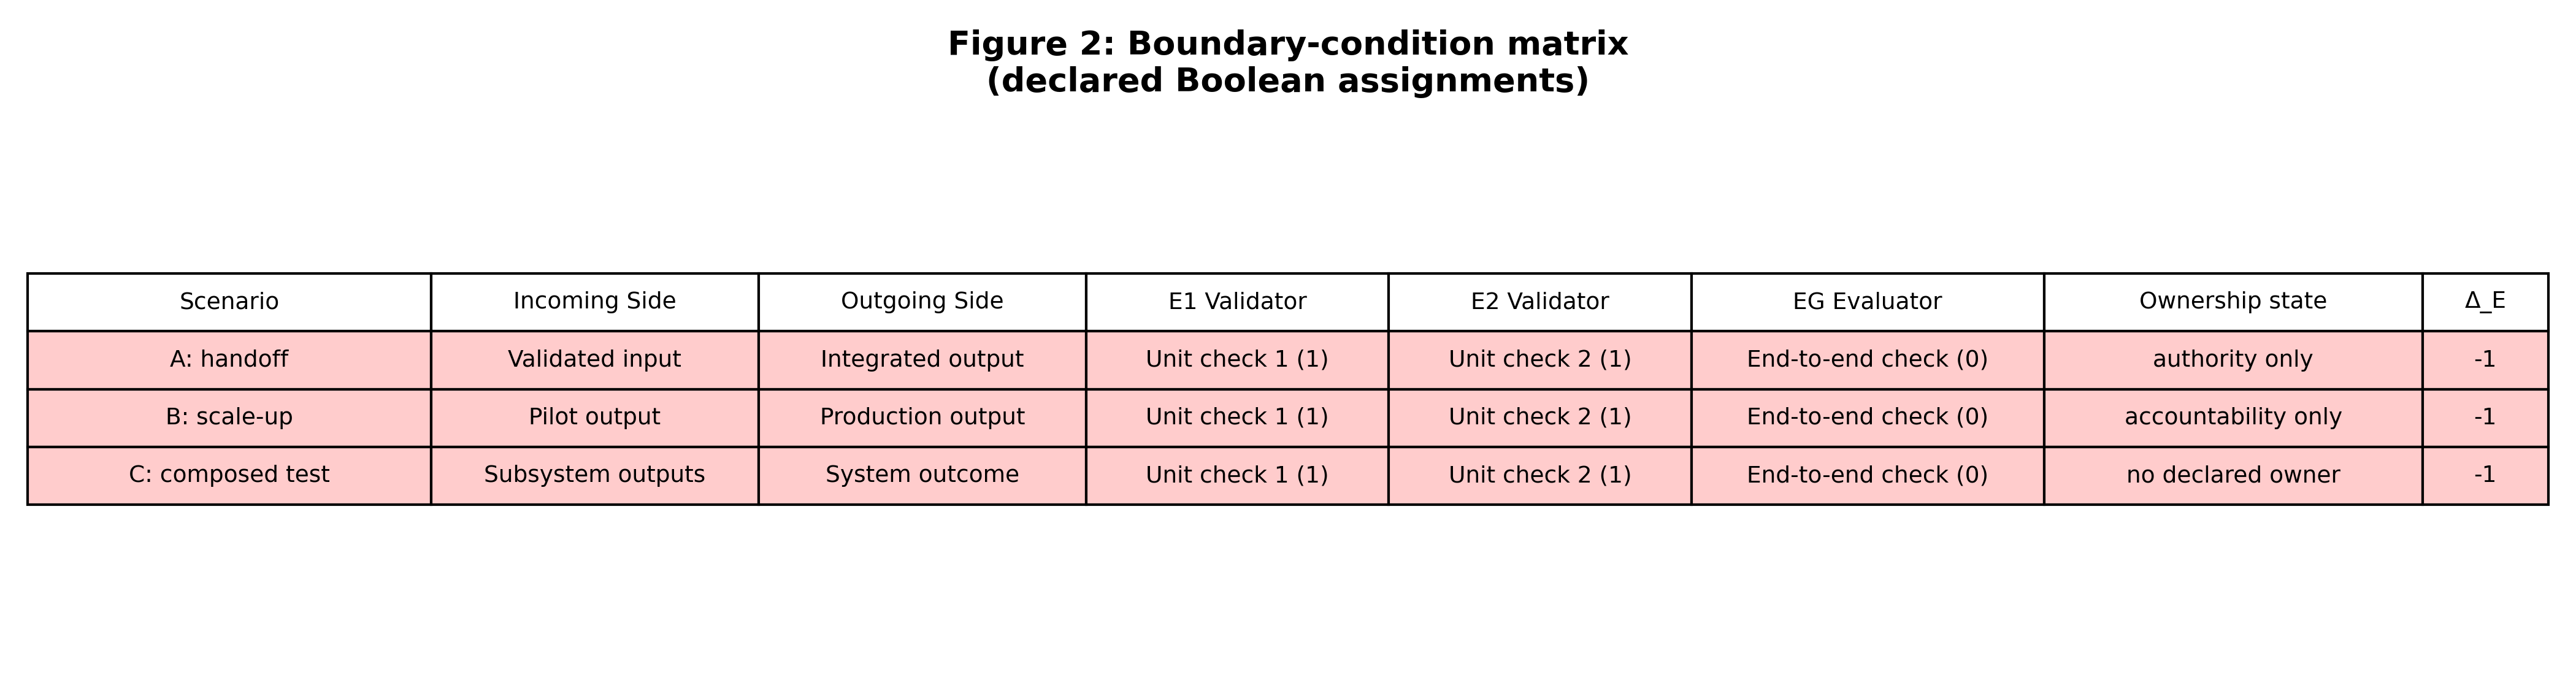
\includegraphics[keepaspectratio,alt={Governance conditions and finite audit matrix}]{public_export/figure_2_case_studies_defect_matrix.png}}
\caption{Governance conditions and finite audit matrix}
\end{figure}

\newpage

\subsection{5. Executable evidence}\label{executable-evidence}

\subsubsection{5.1 Python}\label{python}

\texttt{code/organizational\_gluing\_core.py} implements the finite data
model, the defect arithmetic, governance conjunction, collapse check,
diagnostic records, and Shapley calculation. Evaluator callbacks accept
only exact Python \texttt{bool} values: numeric stand-ins such as
\texttt{0}, \texttt{1}, \texttt{0.0}, and \texttt{1.0} are rejected.
Valid verdicts are encoded as integer (0/1) values in defect records.
Constructors also reject inconsistent records.

The twelve break-and-recover tests cover nine fault families:

\begin{enumerate}
\def\labelenumi{\arabic{enumi}.}
\tightlist
\item
  non-Boolean local and global verdicts;
\item
  missing ownership or one-sided ownership;
\item
  malformed boundary tokens;
\item
  a collapsing detector;
\item
  a zero-defect claim without adequacy evidence;
\item
  an additive range overflow;
\item
  the weak-sufficiency counterexample;
\item
  a temporal mismatch; and
\item
  an attempted evidence-level escalation.
\end{enumerate}

Each mutation must meet its intended guard before the corrected input is
accepted. Across the two production modules, the release gate separately
requires at least 95 percent line/statement coverage and 95 percent
branch coverage.

\subsubsection{5.2 Lean 4}\label{lean-4}

The nested \texttt{lean4/} project builds five paper-facing modules:

\begin{itemize}
\tightlist
\item
  \texttt{01\_certified\_closure.lean}: governance conjunction and owner
  necessity;
\item
  \texttt{02\_boundary\_sufficiency.lean}: weak-sufficiency
  counterexample and product equivalence;
\item
  \texttt{03\_non\_additivity.lean}: defect range, trichotomy, and
  non-additivity;
\item
  \texttt{04\_carrier\_boundary\_obstruction.lean}: carrier transport
  and quotient obstruction; and
\item
  \texttt{05\_detector\_adequacy.lean}: collapsing and zero-defect
  counterexamples.
\end{itemize}

\texttt{check\_axioms.lean} names every declaration cited in this paper.
The package contains no \texttt{sorry} or \texttt{admit} token. The
axiom report is expected to be empty except for \texttt{Quot.sound}
where quotient equality is used.

The compact labels \textbf{M1--M9} and \textbf{D1} used in the prose
resolve to exact, fully qualified Lean declarations in the claim ledger
and the canonical \texttt{docs/lean\_claim\_map.md}. The
machine-readable companion is \texttt{docs/claim\_code\_map.yaml}.

\subsubsection{5.3 Notebook and figures}\label{notebook-and-figures}

The single public notebook begins with the four-line truth table,
introduces the governance conditions, lets a reader vary all seven
Boolean inputs with widgets, draws the defect landscape, and finishes
with counterexamples and a bad-input recovery exercise. A pytest case
executes every cell headlessly. The publication figures are regenerated
by \texttt{code/generate\_figures.py} under the non-interactive
Matplotlib backend.

\subsection{6. Scope}\label{scope}

The paper establishes finite mathematical and implementation claims
only. Its included scenarios are illustrative Boolean assignments; they
are not audits, predictions, or findings about any organization.

\subsection{7. Related work}\label{related-work}

The local-to-global vocabulary follows the broad gluing perspective used
by Abramsky and Brandenburger, while the mathematical object here is a
much simpler Boolean evaluator model. The organizational reading is
compatible with Conway's observation that communication structure shapes
designed systems. Shapley attribution appears only as a standard
optional analysis of a declared coalitional value function.

\subsection{References}\label{references}

\begin{enumerate}
\def\labelenumi{\arabic{enumi}.}
\tightlist
\item
  Abramsky, S., and Brandenburger, A. ``The Sheaf-Theoretic Structure of
  Non-Locality and Contextuality.'' \emph{New Journal of Physics} 13
  (2011),

  \begin{enumerate}
  \def\labelenumii{\arabic{enumii}.}
  \setcounter{enumii}{113035}
  \tightlist
  \item
    \href{https://doi.org/10.1088/1367-2630/13/11/113036}{doi:10.1088/1367-2630/13/11/113036}
  \end{enumerate}
\item
  Conway, M. E. ``How Do Committees Invent?'' \emph{Datamation} 14(4)
  (1968), 28--31.
  \href{https://melconway.com/Home/pdf/committees.pdf}{Author-hosted
  scan}.
\item
  Shapley, L. S. ``A Value for n-Person Games.'' In \emph{Contributions
  to the Theory of Games II}, Annals of Mathematics Studies 28,
  307--318. Princeton University Press, 1953.
  \href{https://doi.org/10.1515/9781400881970-018}{doi:10.1515/9781400881970-018}
\end{enumerate}

\end{document}
